%+--------------------------------------------------------
%| planar.tex
%|    Specification of planar map
%|
%| by Iddo Hanniel ,Eyal Flato, Dan Halperin, Sariel Har-Peled, 
%| Oren Nechushtan and Shai Hirsch
%+----------------------------------------------------------------------------80
%| update log
%|
%| 01 Jun 2000 - Shai Hirsch
%|    Reference parts taken out into planar_ref.tex
%|
%| 03 May 2000 - Shai Hirsch
%|    Transforming to usage of new cc macros.
%|
%| 06 Apr 2000 - Oren Nechushtan
%|    Documentation for the new Planar map (with bounding box).
%|
%| 30 Mar 2000 - Shai Hirsch
%|    Transforming to new format: Separating to User Manual
%|    and Reference Manual. Using new cc commands.
%|     
%-----------------------------------------------------------------------------80

\def\Ipe#1{\def\IPEfile{#1}\input{#1}}

\renewcommand{\Re}{{\rm I\!\hspace{-0.025em} R}}

\def\C{{\cal C}}
\def\G{{\cal G}}
\def\F{{\cal F}}
\def\I{{\cal I}}
\def\U{{\cal U}}
\def\M{{\cal M}}
\def\eps{{\varepsilon}}
\def\bd{{\partial}}
\def\dm{{\cal D}}

\chapter{Planar Map}
\label{I1_ChapterPlanarMap}

% +========================================================================+
\section{Introduction}
% +========================================================================+
\label{PM_sec:intro}

In this chapter we introduce the \ccc{planar map} which is an
embedding of a \ccc{topological map} into the plane.
It is derived
from the topological map class with additional geometric considerations
and functionalities (e.g., point location, bounding box). 
In this section we briefly review
the geometric concepts added in the planar map; the combinatorial concepts were
reviewed in Chapter ~\ref{I1_ChapterTopologicalMap}, {\em Topological Map}.
We also describe the additional functionality of \ccc{Planar_map_2<Dcel,Traits>}
over that of \ccc{Topological_map<Dcel>}.

\paragraph{Curve:}
We will use the term {\it curve} to describe the image of a continuous
$1\!\!-\!\!1$ mapping into the plane of any one of the following: the
closed unit interval (arc), the open unit interval (unbounded curve),
or the unit circle (closed curve). In all cases a curve is non
self-intersecting. Segments, lines, rays, conic sections are examples for curves.

\paragraph{$x$-Monotone curve:}
We
use a convention2
that a curve $c$ is $x$-monotone if $c$ either intersects 
any vertical line in at most one point, or $c$ is a vertical
segment. 

\paragraph{Planar subdivision (planar map):}
A planar subdivision (or planar map) is an embedding of a planar 
%graph $G$
topological map $T$ 
into the plane, such that each edge of $T$ is embedded as a
bounded $x$-monotone curve and each vertex is embedded as a planar point.
% The image of a vertex of $T$ is a {\em vertex},
%and the image of an arc is an {\em edge}.
In this embedding no
%pair of edges intersect in their interiors.
edge intersects another edge interior.

A {\em face} of the subdivision is a maximal connected region of the
plane that does not contain any vertex or edge. 
We consider a face to be open, and its boundary is
formed by vertices and halfedges of the subdivision.
The halfedges are oriented around a face so that the face they bound
is to their left. This means that halfedges on the outer boundary
of a face are traversed in counterclockwise order, and halfedges on the inner
boundaries (holes) of a face are traversed in clockwise order. Halfedges 
around a vertex are also traversed in clockwise order. 

\paragraph{Maps with infinite objects (bounding boxes):}

The Planar map deals both with bounded objects, such as segments, circles.
and with infinite objects, such as lines, rays, parabolas.
For simplicity we decided that the default would be the former, e.g. bounded objects.
In order to deal with the latter, some finite representation of such infinite curves is required. The bounding box strategy supplies the required functionality to do this.

A bounding box is defined by two main aspects: its traits representation and its maintenance strategy.
The traits representation is a given shape that corresponds to a region in the plane in which we are interested at a given moment, e.g. a rectangle, a big disk, the whole plane.
The maintenance strategy, can be of many types. The strategy may be of \ccc{static} type , i.e. we are interested only in a fixed region of the plane, curves outside this region are ignored, or it may be \ccc{dynamic}, i.e. the bounding box increases or decreases while the user updates the planar map.
The strategy may be of an \ccc{open} type, i.e. the boundary of the box should not be included as curves of the map, or it may be \ccc{closed}, where this means that the boundary is a part of the planar map.

\paragraph{Point Location:}

Some of the basic operations on planar maps are queries such as ``what is the location of a point in the map?'', or ``which curve is vertically above the point?''.
These geometric queries are supplied as part of this Planar Map class, with 
several algorithms available for the user to choose from.

\paragraph{IO functions:}
IO functions as reading Planar map from the standard input, writing it to the standard output or drawing it to a graphic stream are also provided.

\subsection*{Functionality}

The class \ccc{Planar_map<Dcel,Traits>}  supplies the ability to maintain
a planar map. All the combinatorial entities have a geometric mapping, e.g.,
a vertex of a planar map has a \ccc{Point} data member, a halfedge has
a \ccc{X_curve} (x-monotone curve) data member, etc. In addition to the 
modifying function, namely, insertion, removal, splitting and merging, the user
can perform point location queries and vertical ray shoot queries.
For a full reference of the class (i.e its associated types,
its operations, etc.) read the \ccc{Planar_map Reference Pages}\lcTex{
(\ccRefPage{Pm_Ref_intro})}.

% +========================================================================+
\section{Example Programs}
% +========================================================================+
\label{PM_sec:example}


\begin{figure}[h]
\begin{ccTexOnly}
    \centerline{
      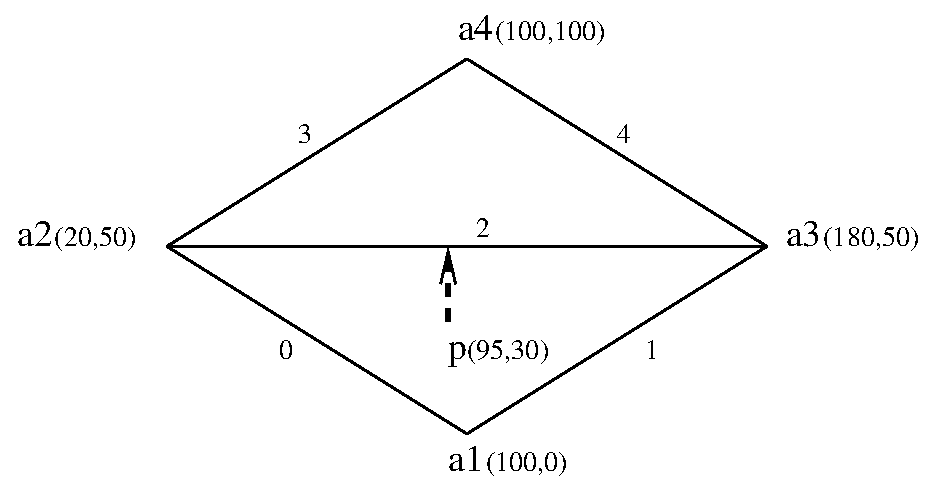
\includegraphics{example_p.ps}
    }
\end{ccTexOnly}

\caption{The map generated by the example program
\label{PM_sec:example_pic}}

\begin{ccHtmlOnly}
    <P>
    <center>
        <img src="example_p.gif"  border=0 alt="example output">
        <!--The map generated by the example program-->
    </center>
\end{ccHtmlOnly}
\end{figure}

The following program creates a planar map from five curves (see
figure ~\ref{PM_sec:example_pic}). It uses the floating-point
arithmetic interface class
(\ccStyle{Pm_segment_epsilon_traits<R>}). The first part of the
code initializes five segments. The next part inserts them into the map
and checks the validity of the map. In the last part, vertical ray
shooting is performed from the point $p$.

% TODO (shai): Change filename to its relative position (3 May 2000)
\ccIncludeExampleCode{Planar_map/example1.C}

The output of the program is

\begin{ccExampleCode}
the curves of the map :
100 0 20 50
100 0 180 50
20 50 180 50
20 50 100 100
180 50 100 100

inserting the curves to the map...
inserting curve0
inserting curve1
inserting curve2
inserting curve3
inserting curve4
check map validity... map valid!

upward vertical ray shooting from 95 30
returned the curve : 20 50 180 50

\end{ccExampleCode}

\subsection{Example of IO functions}
\label{PM_sec:example9}

The following program demonstrates the using of IO functions provided for \ccc{Planar map}.
First the program demonstrates a trivial use of the IO functions, it defines an empty \ccc{Planar map}, then it reads 
the \ccc{Planar map} text from the standard input stream, after the reading it prints to the standard output stream the resulting \ccc{Planar map}.
Second, it presents the use in the verbose format, by defining \ccc{Pm_file_writer} with the verbose flag on, and then call the function \ccc{write_pm}.
Using the interface of the class \ccc{Pm_file_writer} is also presented, by calling to its function \ccStyle{write_halfedges} which prints all the halfedges.
In addition, the program presents in commented lines the operators writing the resulting \ccc{Planar map} to graphic streams, the comments can be removed if the user has LEDA installed. 

\ccIncludeExampleCode{Planar_map/example9.C}

The input of the program is a text file presenting the \ccc{Planar map}. This text file is exactly the same as the first block in the 
output file.
 
%\ccIncludeExampleCode{Planar_map/example9.cin}

The output is the \ccc{Planar map} written in both formats, non verbose and verbose. In addition the two lists 
(non verbose and verbose) of halfedges are written.
\ccIncludeExampleCode{Planar_map/example9_output.txt}

%% EOF %%














